\documentclass[xcolor=x11names]{beamer}
%%%%%%%%%%%%%%%%%%%%%%%%%%%%%%%%%%%%%%%%%%%%%%%%%%%%%%%%%%%%
%%  This Beamer template was created by Cameron Bracken.
%%  Anyone can freely use or modify it for any purpose
%%  without attribution.
%%
%%  Last Modified by C. Bracken: January 9, 2009
%%
%%  The preamble, and maybe some modification of the Cameron Bracken's template is due to Attila Molnár.
%%
%%

%% General document
\usepackage[utf8]{inputenc}
\usepackage[T1]{fontenc}
\usepackage{graphicx}
\usepackage{tikz}
\usetikzlibrary{decorations.fractals}
\usetikzlibrary{decorations.text}
\usepgflibrary{arrows}
\usetikzlibrary{fadings}
\usetikzlibrary[decorations.pathmorphing]
\tikzfading[name=fade inside, inner color=transparent!70, outer color=transparent!70]
\usetikzlibrary{calc}
\usetikzlibrary{intersections}
\usetikzlibrary{shapes}
\usetikzlibrary{patterns}
\usefonttheme{serif}
\usepackage{amssymb} 			
\usepackage{amsmath}
\usepackage{ifthen}
\usepackage[normalem]{ulem}
\usepackage{mathrsfs}

%%%%%%%%%%%%%%%%%%%%%%%%%%%%%%%%%%%%%%%%%%%%%%%%%%%%%%%%%%%%%%%%%%%%%%%%%%%%%%%%%%%%
%% Beamer Layout %%%%%%%%%%%%%%%%%%%%%%%%%%%%%%%%%%
\useoutertheme[subsection=false,shadow]{miniframes}
\useinnertheme{default}
\usefonttheme{serif}
%\usepackage{txfonts} %Hook for strict implication!
\DeclareSymbolFont{symbolsC}{U}{txsyc}{m}{n}
\DeclareMathSymbol{\strictif}{\mathrel}{symbolsC}{74}
\DeclareMathSymbol{\boxright}{\mathrel}{symbolsC}{128}
\usepackage{palatino}
%\usepackage[uppercase=upright,charter]{mathdesign}

\setbeamerfont{title like}{shape=\scshape}
\setbeamerfont{frametitle}{shape=\scshape}


\setbeamercolor*{lower separation line head}{bg=white!40!DeepSkyBlue3}
\setbeamercolor*{normal text}{fg=black,bg=white}
\setbeamercolor*{alerted text}{fg=red}
\setbeamercolor*{example text}{fg=black}
\setbeamercolor*{structure}{fg=black}

\setbeamercolor*{palette tertiary}{fg=black,bg=white!90!DeepSkyBlue3}
\setbeamercolor*{palette quaternary}{fg=black,bg=black!10}

%\setbeamercolor{block body alerted}{bg=normal text.bg!90!DeepSkyBlue4}
\setbeamercolor{block body}{bg=normal text.bg!95!DeepSkyBlue3}
%\setbeamercolor{block body example}{bg=normal text.bg!90!DeepSkyBlue4}
%\setbeamercolor{block title alerted}{use={normal text,alerted text},fg=alerted text.fg!75!normal text.fg,bg=normal text.bg!90!DeepSkyBlue4}
\setbeamercolor{block title}{bg=normal text.bg!70!DeepSkyBlue3}
%\setbeamercolor{block title example}{use={normal text,example text},fg=example text.fg!75!normal text.fg,bg=normal text.bg!75!DeepSkyBlue4}

\setbeamertemplate{blocks}[rounded][shadow=true]
%\setbeamertemplate{background canvas}[vertical shading][bottom=white,top=structure.fg!25]
%\setbeamertemplate{sidebar canvas left}[horizontal shading][left=white!40!black,right=black]
\setbeamertemplate{itemize items}[circle]
\setbeamercolor*{itemize item}{fg=DeepSkyBlue3}
\setbeamercolor*{itemize subitem}{fg=DeepSkyBlue3}
\setbeamercolor*{itemize subsubitem}{fg=DeepSkyBlue3}
\setbeamertemplate{enumerate items}[circle]
%\setbeamercolor{item projected}{bg=DeepSkyBlue3,fg=black}
\setbeamercolor{item projected}{bg=white,fg=DeepSkyBlue3}
\setbeamercolor*{enumerate item}{fg=DeepSkyBlue3}
\setbeamercolor*{enumerate subitem}{fg=DeepSkyBlue3}
\setbeamercolor*{enumerate subsubitem}{fg=DeepSkyBlue3}

%%%%%%%%%%%%%%%%%%%%%%%%%%%%%%%%%%%%%%%%%%%%%%%%%%


%%%%%%%%%%%%%%%%%%%%%%%%%%%%%%%%%%%%%%%%%%%%%%%%%%%%%%%%%%%%%%%%%%%%%%%%%%%%%%%%%%%%

\newenvironment{defi}[1][]{\begin{block}{\footnotesize \textsc{Definition} \ifthenelse{\equal{#1}{}}{}{\, (#1)}}}{\end{block}}
\newenvironment{prop}[1][]{\begin{block}{\footnotesize \textsc{Proposition} \ifthenelse{\equal{#1}{}}{}{\, (\textsc{#1})}}}{\end{block}}
\newenvironment{lemm}[1][]{\begin{block}{\footnotesize \textsc{Lemma} \ifthenelse{\equal{#1}{}}{}{\, (\textsc{#1})}}}{\end{block}}
\newenvironment{idea}[1][]{\begin{block}{\footnotesize \textsc{Idea} \ifthenelse{\equal{#1}{}}{}{\, (\textsc{#1})}}}{\end{block}}
\newenvironment{rema}[1][]{\begin{block}{\footnotesize \textsc{Remark} \ifthenelse{\equal{#1}{}}{}{\, (\textsc{#1})}}}{\end{block}}
\newenvironment{coro}[1][]{\begin{block}{\footnotesize \textsc{Corollary} \ifthenelse{\equal{#1}{}}{}{\, (\textsc{#1})}}}{\end{block}}
\newenvironment{tete}[1][]{\begin{block}{\footnotesize \textsc{Theorem} \ifthenelse{\equal{#1}{}}{}{\, (\textsc{#1})}}}{\end{block}}
\newenvironment{claim}[1][]{\begin{block}{Claim \ifthenelse{\equal{#1}{}}{}{\, (\textsc{#1})}}}{\end{block}}
%\newenvironment{lemma}[1][]{\begin{block}{Lemma \ifthenelse{\equal{#1}{}}{}{\, (\textsc{#1})}}}{\end{block}}
\newenvironment{question}[1][]{\begin{block}{Question \ifthenelse{\equal{#1}{}}{}{\, (\textsc{#1})}}}{\end{block}}
\newenvironment{rem}[1][]{\begin{block}{Remark \ifthenelse{\equal{#1}{}}{}{\, (\textsc{#1})}}}{\end{block}}
\newenvironment{homework}[1][]{\begin{block}{Homework \ifthenelse{\equal{#1}{}}{}{\, (\textsc{#1})}}}{\end{block}}
\newenvironment{proo}[1][]{\begin{block}{\footnotesize \textsc{Proof} \ifthenelse{\equal{#1}{}}{}{\, (\textsc{#1})}}}{\end{block}}

%%%%%%%%%%%%%%%%%%%%%
%% To evade unnecessary circles, mainly for \cimdia
%%%%%%%%%%%%%%%%%%%%%

\makeatletter
\let\beamer@writeslidentry@miniframeson=\beamer@writeslidentry
\def\beamer@writeslidentry@miniframesoff{%
  \expandafter\beamer@ifempty\expandafter{\beamer@framestartpage}{}% does not happen normally
  {%else
    % removed \addtocontents commands
    \clearpage\beamer@notesactions%
  }
}
\newcommand*{\miniframeson}{\let\beamer@writeslidentry=\beamer@writeslidentry@miniframeson}
\newcommand*{\miniframesoff}{\let\beamer@writeslidentry=\beamer@writeslidentry@miniframesoff}
\makeatother

%%%%%%%%%%%%%%%%%%%%%%%%%%%%%
%%%%%%%%%%%%% END %%%%%%%%%%%
%%%%%%%%%%%%%%%%%%%%%%%%%%%%%


%%%% Formatting Commands

\newcommand{\cimdia}[1] {\miniframesoff \begin{frame}\begin{center}\huge \begin{tabular}{c}#1\end{tabular}\end{center}\end{frame}\miniframeson}
\newcommand{\szakasz}[2][]{\section{#1}\subsection{}\cimdia{#2}}
\newcommand{\bluebullet}{\textcolor{DeepSkyBlue3}{\quad $\bullet$} \,\,}

\newenvironment{frame*}[1][]{\miniframesoff \begin{frame} #1}{\end{frame}\miniframeson}

  % for admissible intersections
  \newcommand{\bigsqcap}{\rotatebox[origin=c]{180}{$\bigsqcup$}}

  % Intelligent curves for tikz:
  % Use it in this way: \gorbe{elejenev}{vegenev}{elejeszog}{elejelendulet}{vegeszog}{vegelendulet};
  \newcommand{\gorbe}[6]{\draw (#1).. controls ([shift=(#3: #4 cm)]#1) and ([shift=(#5: #6 cm)]#2) .. (#2);}
  \newcommand{\gorbefelirattal}[8]{\draw (#1).. controls ([shift=(#3: #4 cm)]#1) and ([shift=(#5: #6 cm)]#2) .. (#2) node[#8] {#7};}

\newcommand{\pipa}{%
\begin{tikzpicture}[green!50!black, thick, scale=.1]
\gorbe{0,1}{2,2}{-80}{1}{225}{.7}
\end{tikzpicture}}

\newcommand{\ellentmondas}
		{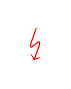
\begin{tikzpicture}[scale=0.2]
			\draw[rounded corners=3pt, rotate=10, red,
					->] (0.75,2)--(0,0.66)--(1,1.33)--(0.25,0);
		\end{tikzpicture}}
\newcommand{\indirektfelteves}
		{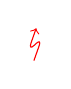
\begin{tikzpicture}[scale=0.2]
			\draw[rounded corners=3pt, rotate=10, red,
					<-] (0.75,2)--(0,0.66)--(1,1.33)--(0.25,0);
		\end{tikzpicture}}

\newcommand{\pecset}[2]{\begin{tikzpicture}[remember picture,overlay]
\node [ draw=red,
        rectangle,
        rounded corners=5mm,
        inner sep=1mm,
        ultra thick,
        fill=white,
        fill opacity=.8,
        rotate=30,
        scale=#1,
        text opacity=0.7]
        at (current page.center)
        {#2};
\end{tikzpicture}}

%\felirat{inner sep}{rounded corners}{scale}{x}{y}{text}
\newcommand{\felirat}[7][]{\begin{tikzpicture}[remember picture,overlay]
\node [draw=DeepSkyBlue3, rectangle, rounded corners=#3 mm, inner sep=#2mm, ultra thick, fill=white, fill opacity=.8, scale=#4, text opacity=1,#1]
at ([xshift=#5 cm, yshift=#6 cm]current page.center) {#7};
\end{tikzpicture}}

\newcommand{\hazi}[6]{\begin{tikzpicture}[remember picture,overlay]
\node [ draw=Coral1,
        rectangle,
        rounded corners=#2 mm,
        inner sep=#1mm,
        ultra thick,
        fill=white,
        fill opacity=.8,
        rotate=0,
        scale=#3,
        text opacity=1]
        at ([xshift=#4 cm, yshift=#5 cm]current page.center)
        {#6};
\end{tikzpicture}}


% Emphasizing:
\definecolor{barna}{rgb}{0.5,0.2,0.1}
\newcommand{\bemph}[1] {{\color{DeepSkyBlue3}{#1}}}
\newcommand{\kemph}[1] {{\color{blue}{#1}}}
\newcommand{\cemph}[1]{\textcolor{red}{#1}}
\newcommand{\zemph}[1] {{\color{Green2}{#1}}}
\newcommand{\yemph}[1] {{\color{Orange1}{#1}}}
\renewcommand{\emph}[1]{\textbf{#1}}

\newcommand{\FD}{\mathbf F}
\newcommand{\FB}{\mathbf G}
\newcommand{\PD}{\mathbf P}
\newcommand{\PB}{\mathbf H}

\newcommand{\FDDot}{\underline{\mathbf F}}
\newcommand{\FBDot}{\underline{\mathbf G}}
\newcommand{\PDDot}{\underline{\mathbf P}}
\newcommand{\PBDot}{\underline{\mathbf H}}


% i dont know whats this
\newcommand{\matbuborek}[1]{%
\begin{tikzpicture}
\node[draw=black, rounded corners=2pt, rectangle, inner sep=1mm] at (0,0){$#1$};
\end{tikzpicture}}


\newcommand{\dzsa}[1]{\textsc{\underline{#1}}:}

% modal operators:
 \newcommand{\diamondmeret}{.18}
 \newcommand{\boxmeret}{4*\diamondmeret/5}


 \newcommand{\mland} [1][.1]{\hspace{#1cm}\textup{and}\hspace{#1cm}}
 \newcommand{\mlthen}[1][.1]{\hspace{#1cm}\Rightarrow\hspace{#1cm}}
 \newcommand{\mlnot} [1][.1]{\hspace{#1cm}\textup{not }}
 \newcommand{\mlor}  [1][.1]{\hspace{#1cm}\textup{or}\hspace{#1cm}}
 \newcommand{\mliff} [1][.1]{\hspace{#1cm}\mliff\hspace{#1cm}}
 \newcommand{\vonal} [1][.2]{\hspace{#1cm} | \hspace{#1cm}}
 \newcommand{\mlwhere} [1][.2]{\hspace{#1cm}\textup{where}\hspace{#1cm}}
 \newcommand{\lrule}[3][c]{\begin{array}{#1} #2  \\  \hline #3 \end{array}}
 \newcommand{\dlrule}[3][c]{\begin{array}{#1} #2  \\  \hline\hline #3 \end{array}}
 \newcommand{\dual}{\delta}
\newcommand{\Dajmond}{\lozenge}
\newcommand{\Boksz}{\square}
\newcommand{\felDajmond}{\blacklozenge}
\newcommand{\felBoksz}{\blacksquare}
\newcommand{\Pmodels}{\mathrel{\models \hspace{-1.8ex} \raisebox{1.1ex}{\scalebox{.5}{$\mathrm{\bemph{P}}$}} }\,}
\newcommand{\Omodels}{\mathrel{\models \hspace{-1.8ex} \raisebox{1.1ex}{\scalebox{.5}{$\mathrm{\bemph{O}}$}} }\,}
\newcommand{\Kmodels}{\mathrel{\models \hspace{-1.8ex} \raisebox{1.1ex}{\scalebox{.5}{$\mathrm{\bemph{K}}$}} }\,}
\newcommand{\Bmodels}{\mathrel{\models \hspace{-1.8ex} \raisebox{1.1ex}{\scalebox{.5}{$\mathrm{\bemph{B}}$}} }\,}
\newcommand{\felle}	
	{\,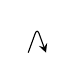
\begin{tikzpicture}
		\pgfmathsetmacro{\szog}{70}
		\pgfmathsetmacro{\hossz}{0.33}
	\draw[->,>=stealth,rounded corners=2pt] (0,0)	--(\szog:\hossz cm)
								--([shift=(-\szog :\hossz cm)]\szog:\hossz cm);	
	\end{tikzpicture}\,}
\newcommand{\lefel}
	{\, 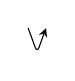
\begin{tikzpicture}
		\pgfmathsetmacro{\szog}{70}
		\pgfmathsetmacro{\hossz}{0.33}
		\draw[->,>=stealth,rounded corners=2pt] (0,0)	--(-\szog:\hossz cm)
								--([shift=(\szog :\hossz cm)]-\szog:\hossz cm);
	\end{tikzpicture}\, }
\newcommand{\enn}
{\mathbf{N}}
\newcommand{\nne}
{\reflectbox{$\mathbf{N}$}}

\newcommand{\mono}{\rightarrowtail}
\newcommand{\epi}{\twoheadrightarrow}
\newcommand{\iso}{\rightarrowtail \!\!\!\!\! \rightarrow}

 \newcommand{\defegy}[1][.1]{\hspace{#1cm}\overset{\textup{\tiny def}}{=}\hspace{#1cm}}
 \newcommand{\defpont}[1][.1]{\hspace{#1cm}\overset{\textup{\tiny def}}{:}\hspace{#1cm}}
 \newcommand{\defekv}[1][.1]{\hspace{#1cm}\overset{\textup{\tiny def}}{ \Leftrightarrow }\hspace{#1cm}}
 \newcommand{\lthen}{\rightarrow}
 \newcommand{\liff}{\leftrightarrow}
 \newcommand{\lminus}{-}
 \newcommand{\lsup}{\mbox{$\mathop{\sim}$}}
 \newcommand{\colnot}{\mbox{$\mathop{\sim}$}}
 \newcommand{\forallin}[2]{(\forall #1 \in #2)}
 \newcommand{\existsin}[2]{(\exists #1 \in #2)}
 \newcommand{\nexistsin}[2]{(\nexists #1 \in #2)}
 \newcommand{\forallp}[1]{(\forall #1)}
 \newcommand{\existsp}[1]{(\exists #1)}
 \newcommand{\forallR}[2]{(\forall #1 \reflectbox{$R$} #2)}
 \newcommand{\existsR}[2]{(\exists #1 \reflectbox{$R$} #2)}
\newcommand{\magyarazat}[2]{\overset{\substack{\textup{#2}\\ \downarrow}}{#1}}
\newcommand{\magyi}[1]{\textup{\bemph{\tiny #1}}}


\newcommand{\bintension}[2][]{{{[}\!{[}} {#2}{{]}\!{]}}^{\mathcal{#1}}}
\newcommand{\wintension}[3][]{{[}\hspace{-.46mm}{[} {#3}{]}\hspace{-.46mm}{]}^{\mathfrak{#1}}_{#2}}
\newcommand{\canintension}[2][]{{[}\hspace{-.46mm}{[} {#2}{]}\hspace{-.46mm}{]}_{\mathrm{#1}}}
\newcommand{\jelentes}[2]{{{[}\!{[}} {#1}{{]}\!{]}}^{{#2}}}
\newcommand{\intension}[2][]{{[}\hspace{-.46mm}{[} {#2}{]}\hspace{-.46mm}{]}^{\mathfrak{#1}}}
\newcommand{\Kintension}[2][]{|\!| {#2} |\!|^{\mathcal{#1}}}
\newcommand{\theory}[2][]{\mathrm{th}_{\mathfrak{#1}}(#2)}
\newcommand{\seenby}{\reflectbox {$R$}}
\newcommand{\derives}[1][]{\vdash_{\mathrm{#1}}}
\newcommand{\ugyanaz}[1]{\mathrel{\overset{#1}{\equiv}}}


\newcommand{\harmasosztas}[6]{

\begin{minipage}{#1\textwidth}%
#4%
\end{minipage}%
\begin{minipage}{#2\textwidth}%
#5%
\end{minipage}%
\begin{minipage}{#3\textwidth}%
#6%
\end{minipage}

}


\newcommand{\felkor}[8]{%
\begin{scope}[draw=#5,very thick,fill opacity=.15,draw opacity=.5,text opacity=1]
\draw[fill=#5]
([shift=(#3:#2)]#1) arc (#3:180+#3:#2) -- cycle;
\node at ([shift=(#7*180+#3:#2),shift=(-#7*90+135+#3:0.5*#6)]#1){#8};
\clip ([shift=(#3:#2)]#1) arc (#3:180+#3:#2);
 \draw[fill=#5] ([shift=(#7*180+#3:#2)]#1) circle (#6);
\end{scope}
}
\newcommand{\felkorvonal}[2]{
\draw[rounded corners=0] (180+#1:.25*#2 cm) arc (180+#1:360+#1:.25*#2 cm)--cycle;
}


\newcommand{\BoxTemplate}[1]{{#1} \mathop{\Box\hspace{-1.35ex} \raisebox{.5ex}{\scalebox{.5}{$\lthen$}}}}
\newcommand{\DiamondTemplate}[1]{#1\hspace{-.2ex} \mathop{\Diamond\hspace{-1.35ex} \raisebox{.4ex}{\scalebox{.5}{$\land$}}}\,}

%%%%%%%%%%%%%%%%%%%%%%%%%%%%%%%%%%%%%%%%%%%%%%%%%%%%%%
\newenvironment{tomb}[2][.1]{\arraycolsep=#1cm\begin{array}{#2}}{\end{array}}
\beamertemplatenavigationsymbolsempty


\author{Attila Moln\'ar}
\date{2014. March 21.}
\title{Axiomatization of Kripkean FOML}
\institute{ELTE}
\begin{document}
\footnotesize


\begin{frame}
\centering
\textsc{\Large Logic of branching time\\[1em] Axiomatizations}

\bigskip

{ \small Attila Moln\'ar

    \textit{E\"otv\"os Lor\'and University}}

 \begin{figure}

\includegraphics[scale=.3]{elte_cimer.png}
 \end{figure}

	\today
\end{frame}

%%%%%%%%%%%%%%%%%%%%%%%%%%%%%%%%%%%%%%%%%%%% NEXT SLIDE %%%%%%%%%%%%%%%%%%%%%%%%%%%%%%%%%%%%%%%%%%%%%

\szakasz[Ockhamist axioms]{Ockhamist axioms}

\begin{frame}
	\frametitle{Ockhamist axiom-checking}

The Lemmon rules, $(\FB\varphi \land \FB \psi )\lthen \FB(\varphi \land \psi )$ and
$(\PB\varphi \land \PB \psi )\lthen \PB(\varphi \land \psi )$ are obvious,

\pause %%%%%%%%%%%%%%%%%% --- PAUSE --- %%%%%%%%%%%%%%%%%%


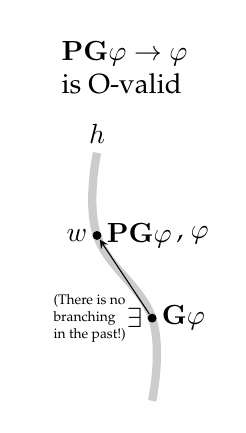
\begin{tikzpicture}[world/.style={inner sep=.4mm, fill=black, circle},>=stealth, scale=.7]

\node at (-0.5,4.5) {\begin{tabular}{l}$\mathbf {PG}\varphi \to \varphi$ \\ is O-valid\end{tabular}};

\node[world] (v2) at (-1,1.5) {};
\node[anchor=south] at (-1,3) {$h$};
\node[anchor=east] at (v2) {$w$};
\draw[opacity=.2, line width=3]  plot[smooth, tension=.7] coordinates {(-1,3) (v2) (0,0) (0,-1.5)};

\pause %%%%%%%%%%%%%%%%%% --- PAUSE --- %%%%%%%%%%%%%%%%%%

\node[anchor=west](felsolabel) at (v2) {$\mathbf{PG}\varphi$};

\pause %%%%%%%%%%%%%%%%%% --- PAUSE --- %%%%%%%%%%%%%%%%%%

\node[world] (v1) at (0,0) {};
\draw[->]  (v1) edge (v2);
\node[anchor=east] at (v1) {$\exists$};
\node[anchor=west] at (v1) {$\mathbf{G}\varphi$};
\node[anchor=east] at (v1) {\tiny \begin{tabular}{l}(There is no \\ branching \\ in the past!)\end{tabular}};

\pause %%%%%%%%%%%%%%%%%% --- PAUSE --- %%%%%%%%%%%%%%%%%%

\node[anchor=west] at (felsolabel) {\quad ,  $\varphi$};
\end{tikzpicture}
\quad
\pause %%%%%%%%%%%%%%%%%% --- PAUSE --- %%%%%%%%%%%%%%%%%%
\uncover<5->{
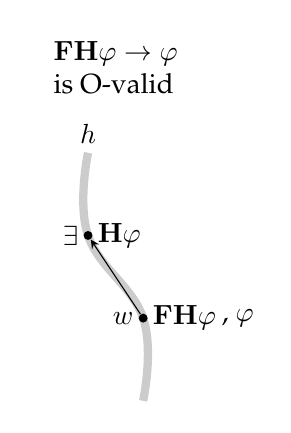
\begin{tikzpicture}[world/.style={inner sep=.4mm, fill=black, circle},>=stealth, scale=.7]

\node at (-0.5,4.5) {\begin{tabular}{l}$\mathbf {FH}\varphi \to \varphi$ \\ is O-valid\end{tabular}};
\node[world] (v1) at (0,0) {};
\node[anchor=south] at (-1,3) {$h$};
\node[anchor=east] at (v1) {$w$};
\draw[opacity=.2, line width=3]  plot[smooth, tension=.7] coordinates {(-1,3) (-1,1.5) (0,0) (0,-1.5)};
\pause %%%%%%%%%%%%%%%%%% --- PAUSE --- %%%%%%%%%%%%%%%%%%
\node[anchor=west](alsolabel) at (v1) {$\mathbf{FH}\varphi$};
\pause %%%%%%%%%%%%%%%%%% --- PAUSE --- %%%%%%%%%%%%%%%%%%
\node[world] (v2) at (-1,1.5) {};
\draw[->]  (v1) edge (v2);
\node[anchor=east] at (v2) {$\exists$};
\node[anchor=west] at (v2) {$\mathbf{H}\varphi$};
\pause %%%%%%%%%%%%%%%%%% --- PAUSE --- %%%%%%%%%%%%%%%%%%
\node[anchor=west] at (alsolabel) {\quad ,  $\varphi$};
\end{tikzpicture}}
\quad
\pause %%%%%%%%%%%%%%%%%% --- PAUSE --- %%%%%%%%%%%%%%%%%%

$\PB \varphi \lthen \PB\PB \varphi$ does the same since the semantics of $\PD$ is the same, this (by the old completeness thm. of K+(4)) implies that we have the validity of $\FB \varphi \lthen \FB\FB \varphi$ as well.

\end{frame}

\begin{frame}
	\frametitle{Ockhamist axiom-checking}
\hspace{-.5cm}\begin{minipage}{10cm}
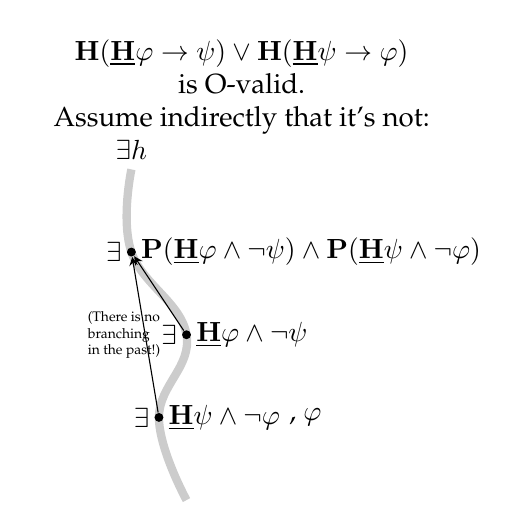
\begin{tikzpicture}[world/.style={inner sep=.4mm, fill=black, circle},>=stealth, scale=.7]

\node at (1,4.5) {\begin{tabular}{c}$\mathbf {H}( \underline {\mathbf H} \varphi \to \psi) \lor \mathbf {H}( \underline {\mathbf H} \psi \to \varphi)$ \\ is O-valid. \\ Assume indirectly that it's not:\end{tabular}};
\node[anchor=south] at (-1,3) {$\exists h$};
\draw[opacity=.2, line width=3]  plot[smooth, tension=.7] coordinates {(-1,3) (-1,1.5) (0,0) (-0.5,-1.5)(-0,-3)};
\node[world] (v2) at (-1,1.5) {};
\node[anchor=east] at (v2) {$\exists$};
\node[anchor=west] at (v2) {$\mathbf {P}( \underline {\mathbf H} \varphi \land \lnot \psi) \land \mathbf {P}( \underline {\mathbf H} \psi \land \lnot \varphi)$};
\pause %%%%%%%%%%%%%%%%%% --- PAUSE --- %%%%%%%%%%%%%%%%%%
\node[world] (v1) at (0,0) {};
\node[anchor=east] at (v1) {$\exists$};
\draw[->]  (v1) edge (v2);
\node[anchor=west] at (v1) {$ \underline {\mathbf H} \varphi \land \lnot \psi$};
\pause %%%%%%%%%%%%%%%%%% --- PAUSE --- %%%%%%%%%%%%%%%%%%
\node[anchor=east] at (v1) {\tiny \begin{tabular}{l}(There is no \\ branching \\ in the past!)\end{tabular}};
\pause %%%%%%%%%%%%%%%%%% --- PAUSE --- %%%%%%%%%%%%%%%%%%
\node[world](v3) at (-0.5,-1.5) {};
\node[anchor=east] at (v3) {$\exists$};
\draw[->]  (v3) edge (v2);
\node[anchor=west](alsolabel) at (v3) {$ \underline {\mathbf H} \psi \land \lnot \varphi$};
\pause %%%%%%%%%%%%%%%%%% --- PAUSE --- %%%%%%%%%%%%%%%%%%
\node[anchor=west] at (alsolabel) {\qquad , $ \varphi$};

\end{tikzpicture}
\pause %%%%%%%%%%%%%%%%%% --- PAUSE --- %%%%%%%%%%%%%%%%%%
\uncover<6->{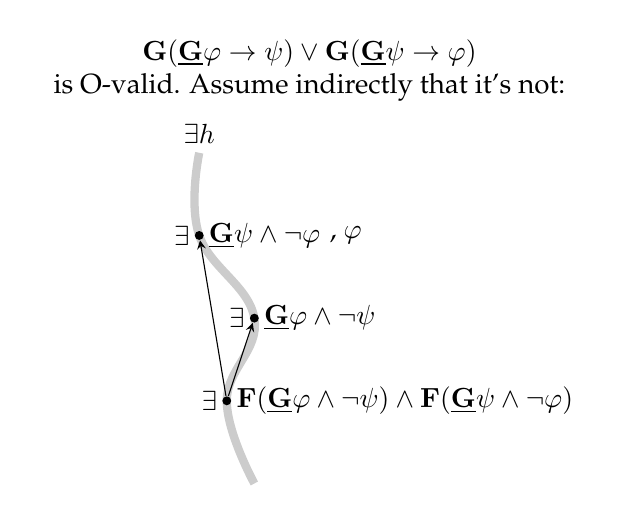
\begin{tikzpicture}[world/.style={inner sep=.4mm, fill=black, circle},>=stealth, scale=.7]
\node at (1,4.5) {\begin{tabular}{c}$\mathbf {G}( \underline {\mathbf G} \varphi \to \psi) \lor \mathbf {G}( \underline {\mathbf G} \psi \to \varphi)$ \\ is O-valid. Assume indirectly that it's not:\end{tabular}};
\node[anchor=south] at (-1,3) {$\exists h$};
\draw[opacity=.2, line width=3]  plot[smooth, tension=.7] coordinates {(-1,3) (-1,1.5) (0,0) (-0.5,-1.5)(-0,-3)};
\node[world](v3) at (-0.5,-1.5) {};
\node[anchor=east] at (v3) {$\exists$};
\node[anchor=west] at (v3) {$\mathbf {F}( \underline {\mathbf G} \varphi \land \lnot \psi) \land \mathbf {F}( \underline {\mathbf G} \psi \land \lnot \varphi)$};
\pause %%%%%%%%%%%%%%%%%% --- PAUSE --- %%%%%%%%%%%%%%%%%%
\node[world] (v1) at (0,0) {};
\node[anchor=east] at (v1) {$\exists$};
\draw[->]  (v3) edge (v1);
\node[anchor=west] at (v1) {$ \underline {\mathbf G} \varphi \land \lnot \psi$};
\pause %%%%%%%%%%%%%%%%%% --- PAUSE --- %%%%%%%%%%%%%%%%%%
\node[world] (v2) at (-1,1.5) {};
\node[anchor=east] at (v2) {$\exists$};
\node[anchor=west](alsolabel) at (v2) {$ \underline {\mathbf G} \psi \land \lnot \varphi$};
\draw[->]  (v3) edge (v2);
\pause %%%%%%%%%%%%%%%%%% --- PAUSE --- %%%%%%%%%%%%%%%%%%
\node[anchor=west] at (alsolabel) {\qquad , $ \varphi$};
\end{tikzpicture}}
\end{minipage}
\end{frame}

\begin{frame}
	\frametitle{``a shot in the dark''}

Since $h\overset w\sim h'$ is an equivalence relation between histories, we should try those axioms for necessity that are valid on equivalence relational frames, i.e., the three axioms of S5:

\begin{itemize}
\item $\Box \varphi \lthen \varphi$ (valid by reflexivity)
\item $\Box \varphi \lthen \Box\Box\varphi$ (valid by transitivity)
\item $\varphi \lthen \Box \Diamond \varphi$ (valid by symmetry)
\end{itemize}

We try to prove the completeness theorem with these. We reserve the right to take new axioms if encounter an appealing formula/rule.

\end{frame}

\begin{frame}
	\frametitle{Trees vs flows}

First of all, if we maintain that the canonical worlds are maximally consistent sets, and the
alternative relation is $\FB^-(\Gamma) \subseteq \Gamma$, then the canonical frame is not one or more tree, but a big union of transitive linear flows (by the validity / axiom status of 4, H.3 and G.3). This is not entirely wrong, since these linear flows with some bulldozing can be good candidates for histories. But how could we make a tree from these histories? The idea will be that we will connect these trees with a new alternative relation, the one which will interpret the historical necessity $\Box$. But then of course this will be a bimodal frame, called Kamp-frame, which is not a usual frame (we have two alternative relation instead of one). But we will show that every Kamp-frame determines a normal frame uniquely, and every normal frame determines a Kamp-frame uniquely.

\end{frame}

\szakasz[Kamp-frames]{Kamp-frames}

\begin{frame}
	\frametitle{Kamp-frames}

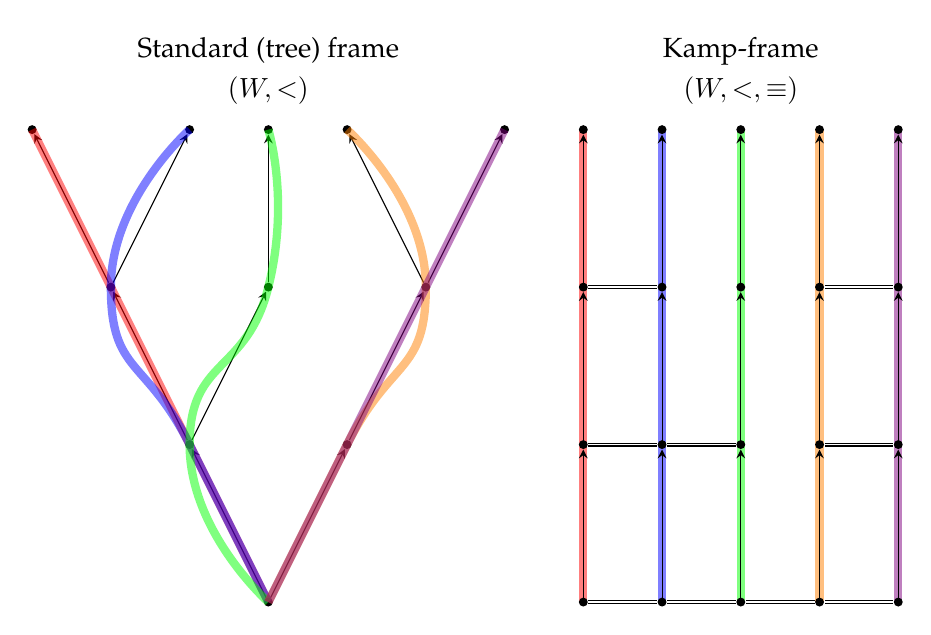
\begin{tikzpicture}[world/.style={inner sep=.4mm, fill=black, circle},>=stealth, scale=1]



\node[world] (v1) at (0,-2) {};
\node[world] (v2) at (-1,0) {};
\node[world] (v3) at (1,0) {};
\node[world] (v4) at (-2,2) {};
\node[world] (v5) at (0,2) {};
\node[world] (v6) at (-3,4) {};
\node[world] (v9) at (2,2) {};
\node[world] (v10) at (1,4) {};
\node[world] (v11) at (3,4) {};
\node[world] (v8) at (0,4) {};
\node[world] (v7) at (-1,4) {};
\draw[->]  (v1) edge (v2);
\draw[->]  (v1) edge (v3);
\draw[->]  (v2) edge (v4);
\draw[->]  (v2) edge (v5);
\draw[->]  (v4) edge (v6);
\draw[->]  (v4) edge (v7);
\draw[->]  (v5) edge (v8);
\draw[->]  (v3) edge (v9);
\draw[->]  (v9) edge (v10);
\draw[->]  (v9) edge (v11);



\begin{scope}[line width=3, opacity=.5]
\draw[red]    plot[smooth, tension=1] coordinates {(v1) (v2) (v4) (v6)};
\draw[blue]   plot[smooth, tension=1] coordinates {(v1) (v2) (v4) (v7)};
\draw[green]  plot[smooth, tension=1] coordinates {(v1) (v2) (v5) (v8)};
\draw[orange] plot[smooth, tension=1] coordinates {(v1) (v3) (v9) (v10)};
\draw[violet] plot[smooth, tension=1] coordinates {(v1) (v3) (v9) (v11)};
\end{scope}

\foreach \x/\color in {1/red,2/blue,3/green,4/orange,5/violet}
{
\draw[line width=3, draw opacity=.5, draw=\color] (3+\x,-2)--(3+\x, 4);
\foreach \y in {0,2,4,6}{\node[world](w\x\y) at (3+\x, \y-2){};}
\foreach \y in {2,4,6}{\draw[->] (3+\x, \y-4) -- (w\x\y);}
}

\begin{scope}
\draw[double] (w10) -- (w20) ;
\draw[double] (w20) -- (w30) ;
\draw[double] (w30) -- (w40) ;
\draw[double] (w40) -- (w50) ;
%%%%%%%%%%%%
\draw[double] (w12) -- (w22) ;
\draw[double] (w22) -- (w32) ;
\draw[double] (w42) -- (w52) ;
%%%%%%%%%%%%
\draw[double] (w14) -- (w24) ;
%\draw (w24) -- (w34) ;
\draw[double] (w44) -- (w54) ;
\end{scope}

\node at (0,5) {Standard (tree) frame};
\node at (6,5) {Kamp-frame};

\node at (0,4.5) {$(W, <)$};
\node at (6,4.5) {$(W, <, \equiv)$};
\end{tikzpicture}
On a Kamp-frame, $<$ is non-branching, while $\equiv$ is an equivalence relation. \\ Think of $\equiv$ as ``is the same as'', or as a rope what we use to make the bundle of histories.
\end{frame}

%%%%%%%%%%%%%%%%%%%%%%%%%%%%%%%%%%%%%%%%%%%%%%%%%%%%%%%%%%%%%%%%%%%%%%%%%%%%%%%%%%%%%%%%%%%%%%%%%%%5

\begin{frame}
	\frametitle{Kamp-frames}

A Kamp-frame is a triplet $(W, <, \equiv)$ where
\begin{itemize}
\item $<$ is irreflexive, transitive and non-branching:
\begin{itemize}
\item $w\not < w$
\item $(w<v \land v<u )\lthen w<u$
\item $(w<v \land w<u) \lthen (v<u\lor v=u\lor v>u)$
\item $(w>v \land w>u) \lthen (v<u\lor v=u\lor v>u)$
\end{itemize}
\item $\equiv$ is reflexive, transitive and symmetric:
\begin{itemize}
\item $w\equiv w$
\item $(w\equiv v \land v\equiv u )\lthen w\equiv u$
\item $w\equiv v \lthen v\equiv w$
\end{itemize}
\item $x \equiv y \lthen x\not <y$ \hfill class irreflexivity
\item $(w \equiv v \land w'<w ) \lthen \existsp {v'<v} \;w'\equiv v'$  \hfill  ``sharing the same past''
\item $\forallp{w,v}\existsp{w'<w}\existsp {v'<v} \;w\equiv v$ \hfill class common root
\item $\forallp{w,v} (w \equiv v \land w\neq v) \existsp{w'>w}\forallp {v'>v} \;w'\not\equiv v'$ \\ \hfill maximality of histories
\end{itemize}

\felirat{1}{1}{.7}{5}{3}{
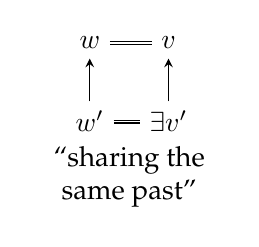
\begin{tikzpicture}[world/.style={inner sep=.4mm, fill=black, circle},>=stealth, scale=1]
\node (v1) at (0,0) {$w'$};
\node (v2) at (0,1) {$w$};
\node (v3) at (1,0) {$\exists v'$};
\node (v4) at (1,1) {$v$};
\draw[->]  (v1) -- (v2);
\draw[->]  (v3) -- (v4);
\draw[double]  (v1) -- (v3);
\draw[double]  (v2) -- (v4);
\node at (0.5,-0.7) {\begin{tabular}{c}``sharing the \\same past''\end{tabular}};
\end{tikzpicture}}
\felirat{1}{1}{.7}{5}{1.125}{
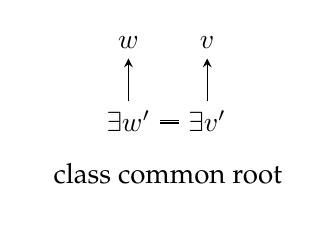
\begin{tikzpicture}[world/.style={inner sep=.4mm, fill=black, circle},>=stealth, scale=1]
\node (v1) at (0,0) {$\exists w'$};
\node (v2) at (0,1) {$w$};
\node (v3) at (1,0) {$\exists v'$};
\node (v4) at (1,1) {$v$};
\draw[->]  (v1) -- (v2);
\draw[->]  (v3) -- (v4);
\draw[double]  (v1) -- (v3);
%\draw[double]  (v2) -- (v4);
\node at (0.5,-0.7) {\begin{tabular}{c}class common root\end{tabular}};
\end{tikzpicture}}
\felirat{1}{1}{.7}{5}{-.75}{
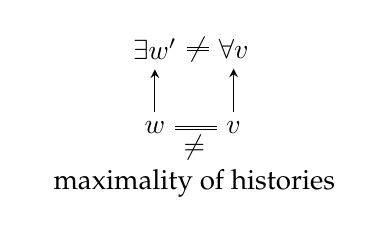
\begin{tikzpicture}[world/.style={inner sep=.4mm, fill=black, circle},>=stealth, scale=1]
\node at (0.5,-0.25) {$\neq$};
\node (v1) at (0,0) {$w$};
\node (v2) at (0,1) {$\exists w'$};
\node (v3) at (1,0) {$v$};
\draw[->]  (v1) -- (v2);
\draw[double]  (v1) -- (v3);
%\pause %%%%%%%%%%%%%%%%%% --- PAUSE --- %%%%%%%%%%%%%%%%%%
\node (v4) at (1,1) {$\forall v$};
\draw[double]  (v2) -- (v4);
\draw[->]  (v3) -- (v4);
\node at (0.5,-0.7) {\begin{tabular}{c}maximality of histories\end{tabular}};
\node at (0.5,1) {$\!\!\!\not$};
\end{tikzpicture}}

\end{frame}

%%%%%%%%%%%%%%%%%%%%%%%%%%%%%%%%%%%%%%%%%%%%%%%%%%%%%%%%%%%%%%%%%%%%%%%%%%%%%%%%%%%%%%%%%%%%%%%%%%%5

\begin{frame}
	\frametitle{Kamp-models}
Let $\mathfrak K=(W, <,\equiv)$ be a Kamp-frame. A Kamp-valuation is a $V:\mathrm{At}\to \wp W$ for which the following additional property holds:
\[ w\in V(p) \Rightarrow \forallp {v\equiv w}\; v\in V(p) \textup{ \qquad for all $p\in \mathrm{At}$} \]
a Kamp-frame $\mathfrak K=(W, <,\equiv)$ together with such a valuation $V$ is a Kamp-model $\mathfrak M_K=(\mathfrak K, V)$.


\[\begin{tomb}[.15]{lcl}
%\textup{Ockhamist:}\\
   \mathfrak M_K , w \Kmodels p &\defekv & w\in V(p)
\\ \mathfrak M_K , w \Kmodels \lnot \varphi &\defekv & \textup{it is not true that }\mathfrak M_K , w \Kmodels \varphi
\\ \mathfrak M_K , w \Kmodels \varphi \land \psi &\defekv & \mathfrak M_K , w \Kmodels \varphi\textup{ and }\mathfrak M_K , w \Kmodels \psi
\\ \mathfrak M_K , w \Kmodels \PD \varphi &\defekv & \existsp {v<w} \; \mathfrak M_K , v \Kmodels \varphi
\\ \mathfrak M_K , w \Kmodels \FD \varphi &\defekv & \existsp {v>w} \; \mathfrak M_K , v \Kmodels \varphi
\\ \mathfrak M_K , w \Kmodels \Diamond \varphi &\defekv & \existsp {v\equiv w} \; \mathfrak M_K, v \Kmodels \varphi
\end{tomb}\]
\end{frame}

%%%%%%%%%%%%%%%%%%%%%%%%%%%%%%%%%%%%%%%%%%%%%%%%%%%%%%%%%%%%%%%%%%%%%%%%%%%%%%%%%%%%%%%%%%%%%%%%%%%5

\begin{frame}
	\frametitle{Models and Kamp-models}
We can transform every Kamp-model $\mathfrak M_K$ into a standard tree-model $\mathrm{str}(\mathfrak M_K)$. Let $\mathfrak M_K=\{W, <, \equiv, V\}$ be a Kamp-model. The \emph{standard transformation} of a Kamp-model $\mathfrak M_K$ will be
\[ \mathrm{str}(\mathfrak M_K) \defegy (W/\equiv, <^{\mathrm{str}}, V^{\mathrm{str}})\]
where
\begin{itemize}
\item $W/{\equiv}$ is the set of all $\equiv$-equivalence classes, i.e.,
\[ W/{\equiv} \defegy \{ w/\equiv \, : \, w \in W \}, \]
where $w/{\equiv} \defegy \{ v\, : \, w\equiv v \}$.
\item $<^{\mathrm{str}}$ is defined as
\[ w/{\equiv} <^{\mathrm{str}} v/{\equiv} \defekv \existsin {w'}{w/{\equiv}}\existsin {v'}{v/{\equiv}} \;w<v \]
\item The valuation of the standard transformed model will be
\[ w/{\equiv} \in V^{\mathrm{str}} (p) \defekv w \in V(p) \]
This definition is correct (does not depend on the choice of $w$) since we used Kamp-valuations, for which it is true that the same atomic sentences are true in equivalent worlds.
\end{itemize}
\end{frame}

\begin{frame}
	\frametitle{Models and Kamp-models}
\dzsa{Proposition} \qquad $(W/\equiv, <^{\mathrm{str}})$ is a tree.

\bigskip

\dzsa{Corollary} \qquad $\mathrm{str}(\mathfrak M_K)$ is a tree model.

\end{frame}


%%%%%%%%%%%%%%%%%%%%%%%%%%%%%%%%%%%%%%%%%%%%%%  NEXT SLIDE %%%%%%%%%%%%%%%%%%%%%%%%%%%%%%%%%%%%%%%%%%%%%%%%%

\begin{frame}[t]
	\frametitle{Models and Kamp-models}
\dzsa{Proposition} \qquad $(W/\equiv, <^{\mathrm{str}})$ is a tree.
\medskip

\hrule

\medskip

\begin{itemize}
\item $<^{\mathrm{str}}$ is irreflexive:
\[\begin{array}{rcll}
   w/{\equiv} \not <^{\mathrm{str}} w/{\equiv}
\pause %%%%%%%%%%%%%%%%%% --- PAUSE --- %%%%%%%%%%%%%%%%%%   & \iff & \lnot \existsin {v,u}{w/{\equiv}}\; v<u &\magyi{ def.of $<^{\mathrm{str}}$}
\pause %%%%%%%%%%%%%%%%%% --- PAUSE --- %%%%%%%%%%%%%%%%%% \\ & \iff & \forallin {v,u}{w/{\equiv}}\; v\not <u &\textup{}
\pause %%%%%%%%%%%%%%%%%% --- PAUSE --- %%%%%%%%%%%%%%%%%% \\ & \iff & v \equiv u \Rightarrow v\not <u&\magyi{``irreflexivity'' of Kamp-frames}
\end{array}\]
\item $<^{\mathrm{str}}$ is transitive:
We have to prove that
\\[-1ex] \quad $\lrule{w/{\equiv}  <^{\mathrm{str}} v/{\equiv} \\ v/{\equiv}  <^{\mathrm{str}} u/{\equiv}}{w/{\equiv}  <^{\mathrm{str}} u/{\equiv}}
\pause %%%%%%%%%%%%%%%%%% --- PAUSE --- %%%%%%%%%%%%%%%%%%
\quad \raisebox{-1.2cm}{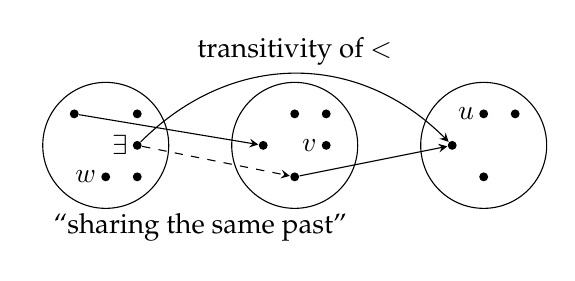
\begin{tikzpicture}[world/.style={inner sep=.4mm, fill=black, circle},>=stealth, scale=.8]

\draw  (0,0) ellipse (1 and 1);
\draw  (3,0) ellipse (1 and 1);
\draw  (6,0) ellipse (1 and 1);

\node[world] (v1) at (-0.5,0.5) {};
\node[world](w) at (0,-0.5) {};
\node[world] at (0.5,0.5) {};
\node[world] at (0.5,-0.5) {};
\node[world] (v2) at (2.5,0) {};
\node[world] (v5) at (3,-0.5) {};
\node[world](v) at (3.5,0) {};
\node[world] (v3) at (3.5,0.5) {};
\node[world] at (3,0.5) {};
\node[world] (v4) at (5.5,0) {};
\node[world] at (6,-0.5) {};
\node[world](u) at (6,0.5) {};
\node[world] at (6.5,0.5) {};

\node[anchor=east] at (w) {$w$};
\node[anchor=east] at (v) {$v$};
\node[anchor=east] at (u) {$u$};

\draw[->]  (v1) edge (v2);
\draw[->]  (v5) edge (v4);
\pause %%%%%%%%%%%%%%%%%% --- PAUSE --- %%%%%%%%%%%%%%%%%%
\node[world] (v6) at (0.5,0) {};
\node[anchor=east] at (v6) {$\exists$};
\draw[->, dashed]  (v6) edge (v5);
\node at (1.5,-1.3) {\begin{tabular}{c}``sharing the same past''\end{tabular}};
\draw  plot[smooth, tension=.7] coordinates {(v6)};
\pause %%%%%%%%%%%%%%%%%% --- PAUSE --- %%%%%%%%%%%%%%%%%%
\draw[->] (v6) .. controls (2,1.5) and (4,1.5) .. (v4);
\node at (3,1.5) {transitivity of $<$};
\end{tikzpicture}}$
\item $<^{\mathrm{str}}$ is rooted:
\end{itemize}
\end{frame}

%%%%%%%%%%%%%%%%%%%%%%%%%%%%%%%%%%%%%%%%%%%%%%%%%%%%%%%%%%%%%%%%%%%%%%%%%%%%%%%%%%%%%%%%%%%%%%%%%%%5

\begin{frame}[t]
	\frametitle{Models and Kamp-models}
\dzsa{Proposition} \qquad $(W/\equiv, <^{\mathrm{str}})$ is a tree.
\medskip

\hrule

\medskip

\begin{itemize}
\item $<^{\mathrm{str}}$ is rooted:
\[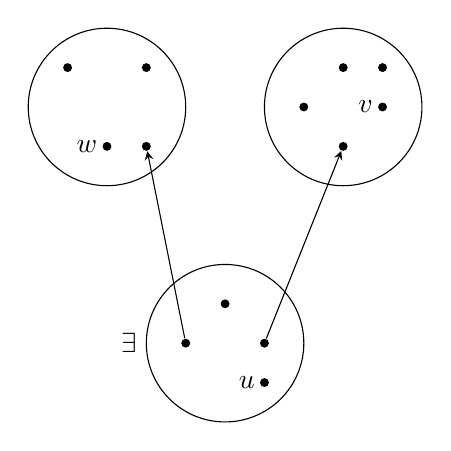
\begin{tikzpicture}[world/.style={inner sep=.4mm, fill=black, circle},>=stealth, scale=1]

\draw  (0,0) ellipse (1 and 1);
\draw  (3,0) ellipse (1 and 1);

\node[world] (v1) at (-0.5,0.5) {};
\node[world](w) at (0,-0.5) {};
\node[world] at (0.5,0.5) {};
\node[world] (v6) at (0.5,-0.5) {};
\node[world] (v2) at (2.5,0) {};
\node[world] (v5) at (3,-0.5) {};
\node[world](v) at (3.5,0) {};
\node[world] (v3) at (3.5,0.5) {};
\node[world] at (3,0.5) {};
\node[anchor=east] at (w) {$w$};
\node[anchor=east] at (v) {$v$};
\draw  (1.5,-3) ellipse (1 and 1);
\node[anchor=east] at (0.5,-3) {$\exists$};
\node[world] (v4) at (1,-3) {};
\node[world] at (1.5,-2.5) {};
\node[world](u) at (2,-3.5) {};
\node[world] (v7) at (2,-3) {};
\node[anchor=east] at (u) {$u$};
\draw[->]  (v4) edge (v6);
\draw[->]  (v7) edge (v5);
\end{tikzpicture}\]

This is equivalent with the Kamp-frame constraint we labelled with ``there is a common root''.
\end{itemize}
\end{frame}

\begin{frame}
	\frametitle{Models and Kamp-models}
Now we should prove something like this:

\[\mathfrak M_K, w \models \varphi \quad \iff \quad \mathrm{str}(\mathfrak M_K), h_w, w/{\equiv} \Omodels \varphi\]
\\ where $h_w$ is defined to be the set of those equivalence classes that contains an element related with $w$:
\[ h_w\defegy \{ v/{\equiv} \, :\, \existsin u{v/{\equiv}} \big(w<u \lor w>u \big) \} \]
$h_w$ will be linear subset because the Kamp-frame's $<$ is always non-branching. It is maximally linear by the way we defined it.

\bigskip

\hazi{2}{1}{.7}{0}{-3.5}{\begin{minipage}{10cm}
\begin{itemize}
\item $w\equiv v$ implies ${h_w\overset{w/{\equiv}}\sim h_v}$
\item $w\equiv v$ is not implied by ${h_w\overset{w/{\equiv}}\sim h_v}$
\item there is an $u\equiv w$, s.t. $u<v$ or $u>v$, if ${h_w\overset{w/{\equiv}}\sim h_v}$
\end{itemize}
\end{minipage}}

\end{frame}


%%%%%%%%%%%%%%%%%%%%%%%%%%%%%%%%%%%%%%%%%%%%%%  NEXT SLIDE %%%%%%%%%%%%%%%%%%%%%%%%%%%%%%%%%%%%%%%%%%%%%%%%%

\begin{frame}
	\frametitle{Truth in Models and Kamp-models}
Now the problem will be that
\[\mathfrak M_K, w \models \varphi \quad \iff \quad \mathrm{str}(\mathfrak M_K), h_w, w/{\equiv} \Omodels \varphi\]
\cemph{is not true in general.}

\bigskip


It is true when the Kamp-frame is made from a real tree's all histories, but not every Kamp-frame is can be gained from a tree's all histories. Correspondingly, Kamp-validity does not correspond to Ockhamist validity. That is not entirely surprising, since Kamp-frames \emph{cheat} in the interpretation of $\Diamond$: Originally $\Diamond$ quantified over histories, i.e., \emph{sets} of possible worlds. But in a Kamp-frame, $\Diamond$ quantifies over only possible worlds. And it can be the case that there are more histories than worlds. (Although this was not the case in our \emph{finite} examples; in finite examples, the validity of the two are the same.)

\bigskip

But before we introduce the corresponding structure for Kamp-frames, let us find out how far we can get by the proof of the statement above.

\end{frame}

%%%%%%%%%%%%%%%%%%%%%%%%%%%%%%%%%%%%%%%%%%%%%%%%%%%%%%%%%%%%%%%%%%%%%%%%%%%%%%%%%%%%%%%%%%%%%%%%%%%5

\begin{frame}[t]
	\frametitle{Models and Kamp-models}
\dzsa{Theorem}\qquad  $\mathfrak M_K, w \models \varphi \quad \iff \quad \mathrm{str}(\mathfrak M_K), h_w, w/{\equiv} \Omodels \varphi$
\medskip
\hrule
\medskip
the atomic case is
\[\begin{array}{rcll}
\mathfrak M_K, w \models p &\iff &w\in V(p)  &\magyi{def of Kamp-$\models$}
\\ &\iff& w/{\equiv} \in V^{\mathrm{str}}(p) &\magyi{def of $V^{\mathrm{tr}}$}
\\ &\iff& \mathrm{str}(\mathfrak M_K), h_w, w/{\equiv} \Omodels \varphi&\magyi{def of $\Omodels$}
\end{array}\]
the $\land$ and $\lnot$ are trivial by induction, the modal cases are
\[\begin{array}{rcll}
\mathfrak M_K, w \models \FD \varphi &\iff & \existsp {v>w} \mathfrak M_K, v \models \varphi &\magyi{def of Kamp-$\models$}
\\ &\iff& \existsp{v>w} \mathrm{str}(\mathfrak M_K), h_v, v/{\equiv} \Omodels \varphi &\magyi{ind.hip}
\\ &\iff& \existsp{v>w} \mathrm{str}(\mathfrak M_K), h_w, v/{\equiv} \Omodels \varphi &\magyi{$h_w=h_v$ by $w<v$}
\\ &\cemph{\Leftarrow}\!\!\Rightarrow& \existsp{v/{\equiv}>^{\mathrm{str}}w/{\equiv}} \mathrm{str}(\mathfrak M_K), h_w, v/{\equiv} \Omodels \varphi &\magyi{def.of ${<^\mathrm{str}}$}
\\ &\iff& \mathrm{str}(\mathfrak M_K), h_w, w/{\equiv} \Omodels \FD \varphi&\magyi{def of $\Omodels$}
\end{array}\]
here the left direction needs some explanation: From $h_w, w/{\equiv} \Omodels \FD \varphi$ we know that there is an $u/{\equiv}\in h_w$ where $\varphi$ is true, hence by the def. of $h_w$, $\existsin{v}{u/{\equiv}} \; w<u\equiv v$ and we arrived to the third line.

\end{frame}

%%%%%%%%%%%%%%%%%%%%%%%%%%%%%%%%%%%%%%%%%%%%%%%%%%%%%%%%%%%%%%%%%%%%%%%%%%%%%%%%%%%%%%%%%%%%%%%%%%%5

\begin{frame}[t]
	\frametitle{Models and Kamp-models}
\dzsa{Theorem}\qquad  $\mathfrak M_K, w \models \varphi \quad \iff \quad \mathrm{str}(\mathfrak M_K), h_w, w/{\equiv} \Omodels \varphi$
\medskip
\hrule
\medskip
\[\begin{array}{rcll}
\mathfrak M_K, w \models \PD \varphi &\iff & \existsp {v<w} \mathfrak M_K, v \models \varphi &\magyi{def of Kamp-$\models$}
\\ &\iff& \existsp{v<w} \mathrm{str}(\mathfrak M_K), h_v, v/{\equiv} \Omodels \varphi &\magyi{ind.hip}
\\ &\iff& \existsp{v<w} \mathrm{str}(\mathfrak M_K), h_w, v/{\equiv} \Omodels \varphi &\magyi{$h_w=h_v$ by $w<v$}
\\ &\cemph{\Leftarrow}\!\!\Rightarrow& \existsp{v/{\equiv}<^{\mathrm{str}}w/{\equiv}} \mathrm{str}(\mathfrak M_K), h_w, v/{\equiv} \Omodels \varphi &\magyi{def.of ${<^\mathrm{str}}$}
\\ &\iff& \mathrm{str}(\mathfrak M_K), h_w, w/{\equiv} \Omodels \PD \varphi&\magyi{def of $\Omodels$}
\end{array}\]
here the left direction needs the dual argumentation as was presented in the previous slide.
\[\begin{array}{rcll}
\mathfrak M_K, w \models \Diamond \varphi &\iff & \existsp {v\equiv w} \mathfrak M_K, v \models \varphi &\magyi{def of Kamp-$\models$}
\\ &\iff& \existsp{v\equiv w} \mathrm{str}(\mathfrak M_K), h_v, v/{\equiv} \Omodels \varphi &\magyi{ind.hip}
\\ &\iff& \existsp{v\equiv w} \mathrm{str}(\mathfrak M_K), h_v, w/{\equiv} \Omodels \varphi &\magyi{by $\equiv$}
\\ &\iff& \existsp{h_v\overset{w/{\equiv}}\sim h_w} \mathrm{str}(\mathfrak M_K), h_v, w/{\equiv} \Omodels \varphi &\magyi{using the HW.}
\\ &\Rightarrow& \mathrm{str}(\mathfrak M_K), h_w, w/{\equiv} \Omodels \Diamond \varphi&\magyi{def of $\Omodels$}
\end{array}\]

For the other direction we can start with \[\existsp{h\overset{w/{\equiv}}\sim h_w} \mathrm{str}(\mathfrak M_K), h, w/{\equiv} \Omodels \varphi.\]
Now to proceed further, we have to show that this $h$ was already there in the original Kamp-frame. Well, that is not always true.
\end{frame}

%%%%%%%%%%%%%%%%%%%%%%%%%%%%%%%%%%%%%%%%%%% NEXT SLIDE %%%%%%%%%%%%%%%%%%%%%%%%%%%%%%%%%%%%%%%%%%%%%%%%%%%%%%%%5

\begin{frame}[t]
	\frametitle{Counterexample: Infinite binary trees}

\scriptsize
%Consider this grid of those points in the coordinatesystem, whose coordinates are positive integers.
\begin{minipage}{.55\textwidth}
    $W \defegy \{ w : w \textup{ is a route to a point}\}$
\\  $= \{ \langle w_1, \dots , w_n \rangle {:}\, n{\in} \omega, \forallp {i{\leq} n} w_i{\in} \{U,R\}\} $
\\[1em]  $w \sqsubseteq v \defekv \textup{$v$ is a continuation of $w$}$, i.e.,
\\       iff $\forallp {i\leq n} w_i= v_i $ where $n$ is the length of $w$.
\\[1em] Note that histories correspond to infinite routes!
\\[1em] Also note we can not name the histories by worlds (as was the case in the finite cases)! There are (infinitely) many infinite continutations of finite routes.
\\
\begin{minipage}{1.2cm}
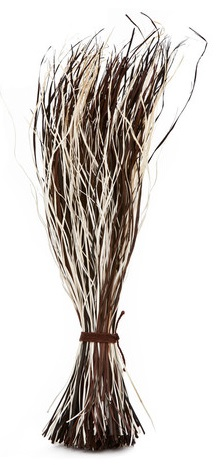
\includegraphics[scale=.15]{kepek/bundle.jpeg}
\end{minipage}
\begin{minipage}{4.5cm}
A set of histories $B\subseteq \mathrm{H}(\mathfrak F)$ is called a \textbf{bundle} iff \[ \bigcup B = W, \]
that is, for every $w\in W$ there is a history $h\in B$ s.t. $w\in h$.
\end{minipage}
\\ We can find a proper bundle, which is in fact can be named by worlds:
\[ \{ h\in \mathrm H(\mathfrak F) : \exists w \forallp {v>w} v=\langle w,U,\dots, U\rangle  \}\]
\end{minipage}
\begin{minipage}{.2\textwidth}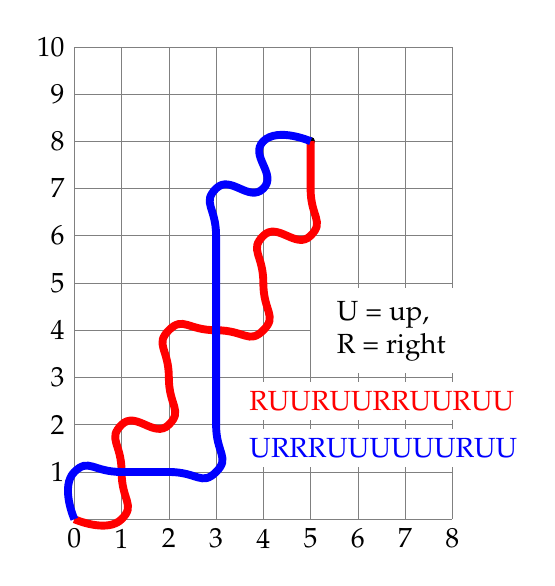
\begin{tikzpicture}[>=stealth, scale=.6,
world/.style={inner sep=.4mm, fill=black, circle},
intension/.style={fill=black, fill opacity=.1},
altrel/.style={->}]


%%%%%% SETTINGS %%%%%%%%%%

\pgfmathtruncatemacro{\gridwidth}{8}
\pgfmathtruncatemacro{\gridheight}{10}

%%%%%% RAJZ %%%%%%%%%%

\draw [help lines, step=1cm] (0,0) node (v1) {} grid (\gridwidth,\gridheight);

\foreach \i in {0, ..., \gridwidth}{\node [anchor=north] at (\i, 0) {\i};}
\foreach \i in {1, ..., \gridheight}{\node [anchor=east] at (0,\i) {\i};}

%\pause %%%%%%%%%%%% PAUSE %%%%%%%%%%%%%

\node [world] (v8) at (5,8) {};

%\pause %%%%%%%%%%%% PAUSE %%%%%%%%%%%%%


\begin{scope}[line width=1mm]
\draw[red]  plot[smooth, tension=1.1] coordinates {(v1) (1,0) (1,1) (1,2) (2,2) (2,3) (2,4) (3,4) (4,4) (4,5) (4,6) (5,6) (5,7) (v8)};
%\pause %%%%%%%%%%%% PAUSE %%%%%%%%%%%%%
\draw[blue]  plot[smooth, tension=1.1] coordinates {(v1) (0,1) (1,1) (2,1) (3,1) (3,2) (3,3) (3,4) (3,5) (3,6) (3,7) (4,7) (4,8) (v8)};
\end{scope}

%\pause %%%%%%%%%%%% PAUSE %%%%%%%%%%%%%


\begin{scope}[fill=white, anchor=west]
\node[fill=white, text=red] at (3.5,2.5) {RUURUURRUURUU};
\node[fill=white, text=blue] at (3.5,1.5) {URRRUUUUUURUU};
\node[fill=white, text=black] at (5,4) {\begin{tabular}{l}U = up,\\ R = right\end{tabular}};
\end{scope}

\end{tikzpicture}\end{minipage}
\end{frame}

%%%%%%%%%%%%%%%%%%%%%%%%%%%%%%%%%%%%%%%%%%% NEXT SLIDE %%%%%%%%%%%%%%%%%%%%%%%%%%%%%%%%%%%%%%%%%%%%%%%%%%%%%%%%5


\begin{frame}[t]
	\frametitle{Bundled trees}
\scriptsize

\dzsa{Definition} A bundled tree is a triplet $(W, <, B)$ where $(W,<)$ is a tree and $B\subseteq \mathrm{H}(W, <)$ is a bundle.

\bigskip

\dzsa{Proposition} Every bundled tree can be ``turned into'' a Kamp-frame.

\bigskip

\dzsa{Proposition} Validity on Kamp-frames correspond to the validity on bundled trees.

\end{frame}


\begin{frame}[t]
	\frametitle{Workshop project}

Invent a transformation $\mathrm{rts}$ that goes in the reverse direction: that transforms an arbitrary standard model into a Kamp-model:
\begin{itemize}
\item prove that the resulting frame is always a Kamp-frame, and the resulting valuation is a Kamp-valuation.
\item prove that this transformation preserves the truth.
\item this transformation is indeed the reverse of $\mathrm{str}$, by proving the following statement:
\[ \mathrm{str}(\mathrm{rts}(\mathfrak M)) \simeq \mathfrak M \quad \textup{ and } \quad \mathrm{rts}(\mathrm{str}(\mathfrak M_K))\simeq \mathfrak M_K \]
where $\mathfrak M \simeq\mathfrak M' $ means that there is an $f$ bijection between $W$ and $W'$ s.t.
\[ wRv \iff f(w)R'f(v) \textup{ and } w \in V(p) \iff f(w)\in V'(p)\]
\end{itemize}

\end{frame}


%%%%%%%%%%%%%%%%%%%%%%%%%%%%%%%%%%%%%%%%%%%%%%%%%%%%%%%%%%%%%%%%%%%%%%%%%%%%%%%%%%%%%%%%%%%%%%%%%%%5
\szakasz[O-completeness]{Ockham completeness}
%%%%%%%%%%%%%%%%%%%%%%%%%%%%%%%%%%%%%%%%%%%%%%%%%%%%%%%%%%%%%%%%%%%%%%%%%%%%%%%%%%%%%%%%%%%%%%%%%%%5

\begin{frame}[t]
	\frametitle{Canonical model}
We introduced the Kamp-models because it is easier to create a canonical Kamp-model than a standard tree model, and we have two reasons:
 \begin{itemize}
 \item If we want to maintain our definition of the canonical alternative relation to be $\FB^-(\Gamma)\subseteq \Gamma'$, then the presence of the axioms H.3 and G.3 will force the canonical relation to be non-branching. But we need a tree for a standard model. But in a Kamp model $<$ is nonbranching!
 \item %Note that in the light of the Truth Lemma, the construction of the canonical model is the following: we first define the valuation (by giving the worlds), then the alternative relation is defined based on the valuation (the $\FB^-(\Gamma)\subseteq \Gamma'$ constraint is about what is true in $\Gamma$ and $\Gamma$'). (Note that in general, truth of modal formulas is based on what is the underlying frame, not the other way around!).
     Now we have this thing called history. This history should be present in the truth lemma, so we have to formulate a new lemma. Also the notion of history needs syntactical construction. What should that be? These questions do not arise in Kamp-frames since there are no histories there.
\end{itemize}
\end{frame}

%%%%%%%%%%%%%%%%%%%%%%%%%%%%%%%%%%%%%%%%%%%%%%%%%%%%%%%%%%%%%%%%%%%%%%%%%%%%%%%%%%%%%%%%%%%%%%%%%%%5
%%%%%%%%%%%%%%%%%%%%%%%%%%%%%%%%%%%%%%%%%%%%%%%%%%%%%%%%%%%%%%%%%%%%%%%%%%%%%%%%%%%%%%%%%%%%%%%%%%%5

\begin{frame}[t]
	\frametitle{another shot in the dark}
\scriptsize
So we have the hunch that (Ockhamist) Kamp-frames have the same logic as normal (Ockhamist) tree models. Then we can conjuncture some more axioms.

\bigskip

Remember that the Kamp-valuation had this important defining property:
\[ w\in V(p) \Rightarrow \forall (w'\equiv w)\; w'\in V(p)  \]

The object language can notice this by the validity of the formulas
\[ p\lthen \Box p  \textup{\qquad  \cemph{where $p\in \mathrm{At}$}}\]
Note that of course cannot be true for any formula, only for the atomic ones. (The future tenses make the histories different!) So we have an axiom scheme that is true only for the atomic sentences, but not all sentences. This will cause that some very popular modal properties will fail, e.g. the substitutivity:

\dzsa{Proposition} It is \cemph{not} true that if $\varphi$ is valid (true on every model's every history's every world) then $\varphi[p/\psi]$, the formula which is resulted by substituting every occurrences of $p$ by $\psi$ in $\varphi$, is valid as well.

\hazi{2}{1}{.7}{0}{-3.8}{\begin{minipage}{13cm}
\textbf{Workshop project:}
\begin{itemize}
\item Prove that this theorem was in true in the determinist flow of time logics! (You can find it in the literature, but my opinion is that it is easier to prove it again than find such a proof.)
\item Under what restrictions is that theorem is true?
(like ``$\varphi$ (or $\psi$) has no $\FD$-s (or $\PD$-s) (or $\Diamond$-s), or has at most only the $\FD$ (or $\PD$) (or $\Diamond$) nonclassical operators in it'' -- that is 12 option!)
\item Try to formalize the most general statement(s) using 12 cases.
\end{itemize}
\end{minipage}}
\end{frame}

%%%%%%%%%%%%%%%%%%%%%%%%%%%%%%%%%%%%%%%%%%%%%%%%%%%%%%%%%%%%%%%%%%%%%%%%%%%%%%%%%%%%%%%%%%%%%%%%%%%5
%%%%%%%%%%%%%%%%%%%%%%%%%%%%%%%%%%%%%%%%%%%%%%%%%%%%%%%%%%%%%%%%%%%%%%%%%%%%%%%%%%%%%%%%%%%%%%%%%%%5

\begin{frame}[t]
	\frametitle{Canonical model}
Our \textbf{starting} axiom system is
\[\mathbf {OBT} + \mathrm{(F4)+(\mathrm H.3)+ (\mathrm G.3)+ (T)+(4)+(B)+(aTriv)}\]
\begin{minipage}[t]{5.78cm}
\begin{itemize}
\item[(PC1)] $\varphi \lthen .\psi \lthen \varphi$
\item[(PC2)] $\varphi\lthen (\psi \lthen \chi) \lthen\!\!. (\varphi \lthen \psi) \lthen\!\! . \varphi \lthen \chi$
\item[(PC3)] $\varphi \lthen \psi \lthen .\lnot \psi \lthen \lnot \varphi$
\item[(CP)] $\PD\FB\varphi \lthen \varphi $
\item[(CF)] $\FD\PB\varphi \lthen \varphi$
\item[(AP)] $(\FB\varphi \land \FB \psi )\lthen \FB(\varphi \land \psi )$
\item[(AF)] $(\PB\varphi \land \PB \psi )\lthen \PB(\varphi \land \psi )$
\item[(MP)] $\lrule {\varphi \\ \varphi \lthen \psi}{\psi}$
\item[(Lem)] $\lrule{\varphi\lthen \psi}{\PB\varphi \lthen \PB\psi}$\; $\lrule{\varphi\lthen \psi}{\FB\varphi \lthen \FB\psi}$

\end{itemize}
\end{minipage}\quad
\begin{minipage}[t]{4.5cm}
\begin{itemize}
\item[(F4)] $\FB\varphi\lthen \FB\FB\varphi$
\item[(H.3)] $\PB(\PBDot \varphi\lthen \psi ) \lor \PB(\PBDot \psi\lthen \varphi )$
\item[(G.3)] $\FB(\FBDot \varphi\lthen \psi ) \lor \FB(\FBDot \psi\lthen \varphi )$
\item[(T)] $\Box \varphi \lthen \varphi$
\item[(4)] $\Box \varphi\lthen \Box\Box \varphi$
\item[(B)] $\Diamond \Box \varphi \lthen \varphi$
\item[(aTriv)] $p\lthen \Box p$ where $p$ is atomic
\end{itemize}
\end{minipage}

\felirat{1}{1}{.7}{4}{-3.5}{\begin{minipage}{5cm}It is very likely that we are still missing some axioms/rules since we have no axioms/rules about how the mixed temporal-alethic formulas behaves, i.e., about the $\Diamond$-$\PD$-$\FD$ interplay! \end{minipage}}
\end{frame}
%%%%%%%%%%%%%%%%%%%%%%%%%%%%%%%%%%%%%%%%%%%%%%%%%%%%%%%%%%%%%%%%%%%%%%%%%%%%%%%%%%%%%%%%%%%%%%%%%%%5
%%%%%%%%%%%%%%%%%%%%%%%%%%%%%%%%%%%%%%%%%%%%%%%%%%%%%%%%%%%%%%%%%%%%%%%%%%%%%%%%%%%%%%%%%%%%%%%%%%%5
\begin{frame}
\frametitle{A canonical model of $\mathbf K$}

\[\mathfrak M_{\mathbf {OBT}} \defegy \left( W_{\mathbf {OBT}}, <_{ \mathbf {OBT}}, \equiv_{ \mathbf {OBT}}, V_{\mathbf {OBT}}\right)   \]
where
\begin{itemize}
\item $W_{\mathbf {OBT}} \defegy \{\Gamma \, :\, \textup{$\Gamma$  is a maximally $\mathbf {OBT}$-consistent set} \}$, i.e.,
\item $\Gamma <_{\mathbf {OBT}}\Gamma'$ iff $\Gamma'$ contains $\varphi$ whenever $\Gamma$ contains $\FB \varphi$, formally:
 \[ \Gamma <_{\mathbf {OBT}}\Gamma' \defekv \FB^-(\Gamma )\subseteq \Gamma' \qquad \qquad \textup{ where }\FB^-(\Gamma)\defegy \{\varphi \, : \, \FB \varphi \in \Gamma\}\]
\item $\Gamma \equiv_{\mathbf {OBT}}\Gamma'$ iff $\Gamma'$ contains $\varphi$ whenever $\Gamma$ contains $\Box \varphi$, formally:
 \[ \Gamma \equiv_{\mathbf {OBT}}\Gamma' \defekv \Box^-(\Gamma )\subseteq \Gamma' \qquad \qquad \textup{ where }\Box^-(\Gamma)\defegy \{\varphi \, : \, \Box \varphi \in \Gamma\}\]
\item $\Gamma \in V_{\mathbf {OBT}}(p) \defekv p\in \Gamma$
\end{itemize}
\end{frame}
%%%%%%%%%%%%%%%%%%%%%%%%%%%%%%%%%%%%%%%%%%%%%%%%%%%%%%%%%%%%%%%%%%%%%%%%%%%%%%%%%%%%%%%%%%%%%%%%%%%5
%%%%%%%%%%%%%%%%%%%%%%%%%%%%%%%%%%%%%%%%%%%%%%%%%%%%%%%%%%%%%%%%%%%%%%%%%%%%%%%%%%%%%%%%%%%%%%%%%%%5
\begin{frame}
\frametitle{A canonical model of $\mathbf K$}
\dzsa{theorem} $\mathfrak M_{\mathbf {OBT}}$ is a model.
\medskip
\hrule
\medskip

\begin{itemize}
\item The valuation is Kampian if we have the truth lemma: if $w\in V_{\mathbf {OBT}}(p)$ then $p\in w$, but then since we have the axioms $p\lthen \Box p$ for atomic formulas, and axioms are contained in every canonical worlds, and canonical worlds are closed under the derivation rules, $\Box p\in w$, then by the truth lemma, $\forall v\equiv w\; p\in v$.
\item $<_{\mathbf {OBT}}$ is transitive by the canonicity of $F4$.
\item $<_{\mathbf {OBT}}$ is non-branching by the canonicity of $G.3$ and $H.3$
\item $<_{\mathbf {OBT}}$ is \cemph{not irreflexive}, so we have to \cemph{bulldoze} the clusters later.
\item $\equiv_{\mathbf {OBT}}$ is reflexive by the canonicity of $T$.
\item $\equiv_{\mathbf {OBT}}$ is transitive by the canonicity of $4$.
\item $\equiv_{\mathbf {OBT}}$ is symmetric by the canonicity of $B$.
\end{itemize}

\end{frame}
%%%%%%%%%%%%%%%%%%%%%%%%%%%%%%%%%%%%%%%%%%%%%%%%%%%%%%%%%%%%%%%%%%%%%%%%%%%%%%%%%%%%%%%%%%%%%%%%%%%5
%%%%%%%%%%%%%%%%%%%%%%%%%%%%%%%%%%%%%%%%%%%%%%%%%%%%%%%%%%%%%%%%%%%%%%%%%%%%%%%%%%%%%%%%%%%%%%%%%%%5

\begin{frame}
\frametitle{sharing the same past}

\begin{minipage}{.29 \textwidth} \scriptsize
Suppose that $\Gamma' <_\mathbf{OBT} \Gamma $ and $\Gamma \equiv _\mathbf{OBT} \Sigma$. We have to show that there is a $\Sigma'$ s.t. $\Sigma'<_\mathbf{OBT} \Sigma$ and $\Gamma' \equiv _\mathbf{OBT}\Sigma'$, that is, the situation that is depicted on the right.

To do so, we will show that the set $\Box^-(\Gamma)\cup \mathbf H ^-(\Sigma)$ is consistent, therefore we can extend it to a maximally consistent set $\Sigma'$, which satisfy the properties above since by containing $\Box^-(\Gamma)$ and $\mathbf H ^-(\Sigma)$, it satisfies the (necessary and) sufficient conditions to be connected by the sets $\Gamma'$ and $\Sigma$.

\end{minipage}
\begin{minipage}{.7 \textwidth}
\begin{tikzpicture}[world/.style={inner sep=.4mm, fill=black, circle},set/.style={minimum size=3cm, draw=black, circle},>=stealth, scale=1.4]

\node[set](G) at (0,0) {};
\node[set](S) at (3.5,0) {};
\node[set](G') at (0,-3) {};
\node[minimum size=2cm, draw=black, circle](H-Gamma) at (3.75,-3) {};
\node[minimum size=2cm, draw=black, circle](Box-Gamma) at (3.25,-3) {};

\draw[->]  (G') -- (G)node[sloped, midway, scale=.7, above]{$\mathbf P^+(\Gamma')\subseteq \Gamma$};
\draw[double]  (G) -- (S) node[sloped, midway, scale=.7, above]{$\Gamma\supseteq \Diamond^+(\Sigma)$};

\node at (0.75,1) {$\Gamma$};
\node at (0.75,-2) {$\Gamma'$};
\node at (4.25,1) {$\Sigma$};


\node[scale=.7, anchor=south, inner sep=0] at (2.75,-2.32) {$\Box ^-(\Gamma')$};
\node[scale=.7, anchor=south, inner sep=0] at (4.25,-2.32) {$\mathbf H ^-(\Sigma)$};
\only<1-10>{
\draw  (2.25,-2) rectangle (4.75,-4);
\node[scale=.7, anchor=north] at (3.5,-4) {consequences};
\node[inner sep=0, scale=1](fals) at (4.5,-3.7) {$\bot$};
\only<1>{\draw[->, blue]  (H-Gamma) edge[out=-45, in=135] (fals);}
\draw[->, blue]  (Box-Gamma) edge[out=-45, in=-180] (fals);
\pause %%%%%%%%%%%%%%%%%% --- PAUSE --- %%%%%%%%%%%%%%%%%%
\node[fill=white, fill opacity=.9, draw opacity=.3, scale=1, rounded corners=1pt, draw=black](veges) at (H-Gamma) {$\chi_1, \dots , \chi_n$};
\draw[->, blue]  (veges) edge[out=0, in=90] (fals);
\node[scale=1, blue] at ([yshift=.25cm]S) {$\begin{array}{l}\mathbf H\chi_1, \dots , \mathbf H \chi_n\end{array}$};
\pause %%%%%%%%%%%%%%%%%% --- PAUSE --- %%%%%%%%%%%%%%%%%%
\node[scale=.7](veges2) at (3.5,-3.9) {$\lnot (\chi_1 \land  \dots \land \chi_n)$};
\draw[->, blue]  (Box-Gamma) edge[in=180, out=180] (veges2);

\pause %%%%%%%%%%%%%%%%%% --- PAUSE --- %%%%%%%%%%%%%%%%%% %%%%%%%%%%%%%%%%%% --- PAUSE --- %%%%%%%%%%%%%%%%%%

\node[scale=1] at (G'){$\begin{array}{l}\Box \lnot (\chi_1 \land  \dots \land \chi_n)\end{array}$};

\pause %%%%%%%%%%%%%%%%%% --- PAUSE --- %%%%%%%%%%%%%%%%%%

\node[scale=1] at (0,0.25){$\mathbf P\Box \lnot (\chi_1 \land  \dots \land \chi_n)$};

\pause %%%%%%%%%%%%%%%%%% --- PAUSE --- %%%%%%%%%%%%%%%%%%

\node[scale=1, blue] at (S){$\mathbf H \chi_1 \land  \dots \land \mathbf H \chi_n$};

\pause %%%%%%%%%%%%%%%%%% --- PAUSE --- %%%%%%%%%%%%%%%%%%

\node[scale=1, blue] at ([yshift=-.25cm]S){$\mathbf H (\chi_1 \land  \dots \land \chi_n)$};

\pause %%%%%%%%%%%%%%%%%% --- PAUSE --- %%%%%%%%%%%%%%%%%%

\node[scale=1, blue] at (0,0){$\Diamond \mathbf H (\chi_1 \land  \dots \land \chi_n)$};

\pause %%%%%%%%%%%%%%%%%% --- PAUSE --- %%%%%%%%%%%%%%%%%%

\node[scale=1, blue] at (0,-0.25){$\lnot \Box \mathbf P \lnot (\chi_1 \land  \dots \land \chi_n)$};

\pause %%%%%%%%%%%%%%%%%% --- PAUSE --- %%%%%%%%%%%%%%%%%%

\node[scale=1, red] at (0,-0.5){$\mathbf P \Box \varphi \lthen\Box \mathbf P \varphi $};
}

\pause %%%%%%%%%%%%%%%%%% --- PAUSE --- %%%%%%%%%%%%%%%%%%

\node[red] at (2,-1.5) {$\exists\Sigma'$};
\node[rectangle, minimum width=4cm, minimum height=3.5cm, draw=black, rounded corners=3pt, red](S') at (3.5,-3) {};

\pause %%%%%%%%%%%%%%%%%% --- PAUSE --- %%%%%%%%%%%%%%%%%%

\draw[->, red]  (S') -- (S) node [midway, right, scale=.7]{$\mathbf H^-(\Sigma)\subseteq \Sigma'$};
\pause %%%%%%%%%%%%%%%%%% --- PAUSE --- %%%%%%%%%%%%%%%%%%
\draw[double, red]  (G') -- (S')node [midway, sloped, above, scale=.7]{$\Box^-(\Gamma') \subseteq \Sigma'$};
\end{tikzpicture}
\end{minipage}

\uncover<12>{\pecset{2}{\begin{minipage}{5cm}So if $\mathbf P \Box \varphi \to \Box \mathbf P \varphi$ is an axiom, we can prove the existence of such a $\Sigma'$. But \emph{is it valid}? Because if it is, then it is \emph{canonical} for one of the Kamp-frame properties! \end{minipage}}}
\end{frame}

%%%%%%%%%%%%%%%%%%%%%%%%%%%%%%%%%%%%%%%%%%%%%%%%%%%%%%%%%%%%%%%%%%%%
%%%%%%%%%%%%%%%%%%%%%%%%%%%%%%%%%%%%%%%%%%%%%%%%%%%%%%%%%%%%%%%%%%%%

\begin{frame}
\frametitle{sharing the same past}

The formal derivation:

\[\begin{tomb}{rcll}
   \Box^-(\Gamma')\cup \mathbf H^-(\Sigma) &\vdash  &\bot &\magyi{indirect assumption}
\\ \Box^-(\Gamma') &\vdash  &\lnot (\chi_1 \land \cdots \land \chi_{n}) &\magyi{where {$\Box \chi_i$-s are all in $\Sigma$}}
\\ \Sigma &\vdash  &\Box \lnot (\chi_1 \land \cdots \land \chi_{n}) &\magyi{$\Box^-(\Gamma)\vdash \varphi \Leftrightarrow \Gamma\vdash \Box \varphi$}
\\ \Gamma &\vdash  &\mathbf P \Box\lnot (\chi_1 \land \cdots \land \chi_{n})&\magyi{$\mathbf H^-(\Gamma)\subseteq \Gamma' \Leftrightarrow \mathbf P^+ (\Gamma')\subseteq \Gamma$}
\\ \Gamma &\vdash  &\Box\mathbf P \lnot (\chi_1 \land \cdots \land \chi_{n})&\magyi{THAT WOULD BE GREAT, BECAUSE\dots}
\\ \Sigma &\vdash  &\mathbf P \lnot (\chi_1 \land \cdots \land \chi_{n})& \magyi{$\Box^-(\Gamma)\subseteq \Sigma$}
\\ \Sigma &\vdash  &\lnot \mathbf H (\chi_1 \land \cdots \land \chi_{n})&\magyi{duality}
\\ \Sigma &\vdash  &\lnot (\mathbf H \chi_1 \land \cdots \land \mathbf H\chi_{n})& \magyi{$(\mathbf H \varphi \land \mathbf H \psi) \lthen \mathbf H (\varphi \land \psi)$}
\\ \Sigma &\vdash  &\mathbf H \chi_1 \land \cdots \land \mathbf H\chi_{n}& \magyi{{$\Box \chi_i$-s are all in $\Sigma$!!}}
\end{tomb}\]


\end{frame}

%%%%%%%%%%%%%%%%%%%%%%%%%%%%%%%%%%%%%%%%%%%%%%%%%%%%%%%%%%%%%%%%%%%%%%%%%%%%%%%%%%%%%%%%%%%%%%%%%%%5
%%%%%%%%%%%%%%%%%%%%%%%%%%%%%%%%%%%%%%%%%%%%%%%%%%%%%%%%%%%%%%%%%%%%%%%%%%%%%%%%%%%%%%%%%%%%%%%%%%%5

\begin{frame}
\frametitle{Validity of (HN)}

\[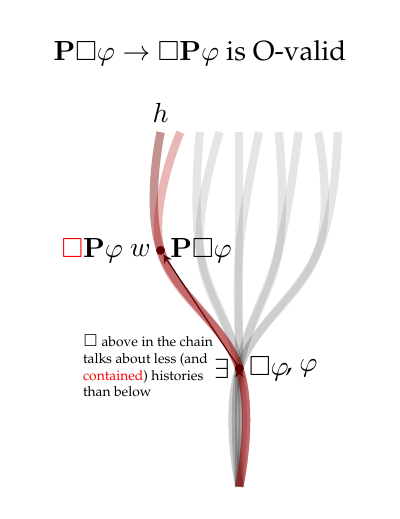
\begin{tikzpicture}[
world/.style={inner sep=.4mm, fill=black, circle},
history/.style={opacity=.2, line width=3},
>=stealth, scale=1]

\node at (-0.5,4) {\begin{tabular}{l}$\mathbf {P}\Box \varphi \to \Box \mathbf P\varphi$ is O-valid\end{tabular}};

\coordinate (alja) at (0,-1.5);
\coordinate (v1) at (0,0);
\node[world] (v2) at (-1,1.5) {};
\coordinate (teteje) at (-1,3);
\node[anchor=south] at (-1,3) {$h$};
\node[anchor=east](vilaglabel) at (v2) {$w$};
\draw[history]  plot[smooth, tension=.7] coordinates {(teteje) (v2) (v1) (alja)};

\pause %%%%%%%%%%%%%%%%%% --- PAUSE --- %%%%%%%%%%%%%%%%%%

\node[anchor=west](felsolabel) at (v2) {$\mathbf{P}\Box \varphi$};

\pause %%%%%%%%%%%%%%%%%% --- PAUSE --- %%%%%%%%%%%%%%%%%%
\node[world] at (v1) {};
\draw[->]  (v1) edge (v2);
\node[anchor=east] at (v1) {$\exists$};
\node[anchor=west](alsolabel) at (v1) {$\Box\varphi$};
\node[anchor=east] at (v1) {\tiny \begin{tabular}{l}$\Box$ above in the chain \\ talks about less (and \\ \textcolor{red}{contained}) histories \\ than below\end{tabular}};

\pause %%%%%%%%%%%%%%%%%% --- PAUSE --- %%%%%%%%%%%%%%%%%%

\node[anchor=west] at (alsolabel) { \ ,  $\varphi$};

\foreach \x in {0,1,2,3,4}
{
\draw[history, opacity=.1]  plot[smooth, tension=.7] coordinates {(alja) (v1) ([xshift=.5*\x cm]v2) ([xshift=.5*\x cm]teteje)};
\draw[history, opacity=.1]  plot[smooth, tension=.7] coordinates {(alja) (v1) ([xshift=.5*\x cm]v2) ([xshift=.5*\x cm,xshift=.25 cm]teteje)};
}

\node[anchor=east] at (vilaglabel) {$\textcolor{red}{\Box} \mathbf{P}\varphi\; $};

\pause %%%%%%%%%%%%%%%%%% --- PAUSE --- %%%%%%%%%%%%%%%%%%

\foreach \x in {0}
{
\draw[history, opacity=.2, red]  plot[smooth, tension=.7] coordinates {(alja) (v1) ([xshift=.5*\x cm]v2) ([xshift=.5*\x cm]teteje)};
\draw[history, opacity=.2, red]  plot[smooth, tension=.7] coordinates {(alja) (v1) ([xshift=.5*\x cm]v2) ([xshift=.5*\x cm,xshift=.25 cm]teteje)};
}


\end{tikzpicture}
\]
\end{frame}

%%%%%%%%%%%%%%%%%%%%%%%%%%%%%%%%%%%%%%%%%%%%%%%%%%%%%%%%%%%%%%%%%%%%%%%%%%%%%%%%%%%%%%%%%%%%%%%%%%%%%%%
%%%%%%%%%%%%%%%%%%%%%%%%%%%%%%%%%%%%%%%%%%%%%%%%%%%%%%%%%%%%%%%%%%%%%%%%%%%%%%%%%%%%%%%%%%%%%%%%%%%%%%%

\begin{frame}
\frametitle{Validity of (HN)}
From now on we refer to $\PD \Box \varphi \lthen \Box \PD \varphi$ as the axiom of historical necessity, or (HN). Now we prove that it is valid on every tree model.

\bigskip

\dzsa{theorem} (HN) is valid on every tree.

\bigskip

\dzsa{proof} Suppose that it is not, i.e., there is a tree model $\mathfrak M$ and a world $w$ on a history $h$ s.t.
\[ \mathfrak M, h, w \Omodels \PD \Box \varphi \qquad \textup{ but not }\qquad
\mathfrak M, h, w \Omodels \Box \PD \varphi.\]
So $\mathfrak M, h, w \Omodels \lnot \Box\PD  \varphi$, i.e., $\mathfrak M, h, w \Omodels \Diamond \PB \lnot \varphi$. This means that there is a history $h' \overset w \sim h$ s.t. $\mathfrak M, h', w \Omodels \PB \lnot \varphi$, and by that we have
\begin{equation} \textup{for all $v<w$ }\qquad  \mathfrak M, h', v \Omodels \lnot \varphi \label{ezzelfogutkozni}
\end{equation}
But our assumption was that $\mathfrak M, h, w \Omodels \PD \Box \varphi$, which means that there is an $u<w$ s.t. $\mathfrak M, h, u \Omodels \Box \varphi$, which implies that $\mathfrak M, h', u \Omodels \varphi$. But this contradicts to (\ref{ezzelfogutkozni}).

\dzsa{theorem} (HN) is valid on every Kamp-model.

\end{frame}



\end{document}
